\documentclass{urdpl}

\usepackage[english,polish]{babel}
\usepackage{polski}
\usepackage[utf8]{inputenc}


\usepackage{mathtools}
\usepackage{amsfonts}
\usepackage{amsmath}
\usepackage{amsthm}
\usepackage[hidelinks]{hyperref}
\usepackage{float}
\usepackage{listings}
\usepackage{graphicx}
\usepackage{booktabs}
\usepackage{multirow} 
\usepackage{tabularx} 
\usepackage{amssymb} 
\usepackage{listings}
\usepackage{xcolor}
\usepackage{array}
\usepackage{afterpackage}
\usepackage{makecell}
\usepackage[flushleft]{threeparttable}
\usepackage[normalem]{ulem}
\usepackage{lineno}
\usepackage{indentfirst}
\usepackage{titlesec}
\usepackage{siunitx}

% ---------------------------------------------
% --- < bibliografia > ---

\usepackage{csquotes}

% ------------------------

% --- < listingi > ---

% Użyj czcionki kroju Courier.
\usepackage{courier}
\usepackage{listings}
\lstloadlanguages{TeX}
\renewcommand{\lstlistlistingname}{Spis listingów}
\renewcommand{\lstlistingname}{Listing}

\lstset{
	literate={ą}{{\k{a}}}1
           {ć}{{\'c}}1
           {ę}{{\k{e}}}1
           {ó}{{\'o}}1
           {ń}{{\'n}}1
           {ł}{{\l{}}}1
           {ś}{{\'s}}1
           {ź}{{\'z}}1
           {ż}{{\.z}}1
           {Ą}{{\k{A}}}1
           {Ć}{{\'C}}1
           {Ę}{{\k{E}}}1
           {Ó}{{\'O}}1
           {Ń}{{\'N}}1
           {Ł}{{\L{}}}1
           {Ś}{{\'S}}1
           {Ź}{{\'Z}}1
           {Ż}{{\.Z}}1,
	basicstyle=\footnotesize\ttfamily,
}

% defnicja stylu JAVA
\lstdefinestyle{javaStyle}{
    language=Java,
    basicstyle=\ttfamily\footnotesize,
    keywordstyle=\color{blue},
    commentstyle=\color{green!50!black}\itshape,
    stringstyle=\color{green},
    numberstyle=\tiny\color{gray},
    numbers=left,
    numbersep=5pt,                      
    stepnumber=1,
    showspaces=false,                  
    tabsize=2,
    showstringspaces=false,
    breaklines=true,
    breakatwhitespace=false,        
    showtabs=false,                    
    keepspaces=true                 
}


\definecolor{stringcolor}{RGB}{163,21,21}   
\definecolor{typecolor}{RGB}{43, 145, 176}   


\definecolor{lightgray}{rgb}{0.9,0.9,0.9}
    \definecolor{green}{rgb}{0,0.6,0}
    \definecolor{gray}{rgb}{0.5,0.5,0.5}

% % ------------------------
\AtBeginDocument{
	\renewcommand{\tablename}{Tabela}
	\renewcommand{\figurename}{Rys.}   
    \newcommand{\listingname}{Listing}
}


% ------------------------
% --- < tabele > ---

% defines the X column to use m (\parbox[c]) instead of p (`parbox[t]`)
\newcolumntype{C}[1]{>{\hsize=#1\hsize\centering\arraybackslash}X}

%---------------------------------------------------------------------------

\author{Dominik Kuraś}
\shortauthor{D. Kuraś}
\noAlbum{134939}

\titlePL{Projekt i implementacja desktopowej aplikacji do zarządzania sklepem z wykorzystaniem języka Java i bazy danych MySQL}
\titleEN{Design and implementation of a desktop application for store management using Java and MySQL}

\shorttitlePL{Aplikacja desktopowa do zarządzania sklepem w Javie} 
\shorttitleEN{Desktop Store Management Application in Java}

\thesistype{Praca projektowa}


\thesisDone{Praca wykonana pod kierunkiem}
\supervisor{mgr inż. Ewa Żesławska}
%\supervisor{mgr inż. Ewa Żesławska}

\degreeprogramme{Informatyka}
%\degreeprogramme{Computer Science}

\date{2025}

\department{Instytut Informatyki}
%\department{Institute of Computer Science}

\faculty{Wydział Nauk Ścisłych i Technicznych}
%\faculty{Faculty of Science and Technology}



\setlength{\cftsecnumwidth}{10mm}

%---------------------------------------------------------------------------
\setcounter{secnumdepth}{4}
\brokenpenalty=10000\relax

% --------------------------------------------------------------------------
% główna część pracy
% --------------------------------------------------------------------------

\begin{document}

\titlepages

% Ponowne zdefiniowanie stylu `plain`, aby usunąć numer strony z pierwszej strony spisu treści i poszczególnych rozdziałów.
\fancypagestyle{plain}
{
    % Usuń nagłówek i stopkę
    \fancyhf{}
    % Usuń linie.
    \renewcommand{\headrulewidth}{0pt}
    \renewcommand{\footrulewidth}{0pt}
}

\setcounter{tocdepth}{2}
\tableofcontents
\clearpage


% dodanie poszczególnych rozdziałów 


\chapter{Streszczenie}
\label{chap:nowe_wprowadzenie}

\section{Streszczenie w języku polskim}
Głównym celem projektu było stworzenie desktopowego systemu do zarządzania sklepem. Aplikacja składa się z dwóch głównych modułów: interfejsu dla klienta (z podziałem na sprzedaż detaliczną i hurtową) oraz panelu dla administratora. System został napisany w języku \textbf{Java}, jego interfejs graficzny powstał przy użyciu biblioteki \textbf{Swing}, a za przechowywanie danych odpowiada baza \textbf{MySQL}. Zastosowanie wzorca projektowego \textbf{DAO} pozwoliło na oddzielenie logiki biznesowej od operacji na bazie danych, co ułatwia utrzymanie i rozwój kodu. Klient może przeglądać produkty i finalizować zakupy, a administrator zarządza asortymentem, klientami, transakcjami i stanami magazynowymi.

\section{Summary in English}
The main objective of this project was to create a desktop store management system. The application consists of two main modules: a customer interface (with separate retail and wholesale functionalities) and an administrator panel. The system was developed in \textbf{Java}, with its graphical user interface built using the \textbf{Swing} library, and a \textbf{MySQL} database for data storage. The use of the \textbf{DAO} design pattern allowed for the separation of business logic from database operations, simplifying code maintenance and scalability. The customer can browse products and complete purchases, while the administrator manages inventory, customers, transactions, and stock levels.
\chapter{Wizja i cele projektu}
\label{chap:wizja}
Celem projektu było stworzenie aplikacji desktopowej, która kompleksowo symuluje działanie sklepu. Wizja zakładała budowę narzędzia, które z jednej strony zapewnia klientom (zarówno detalicznym, jak i hurtowym) \textbf{prostą i wygodną ścieżkę zakupową}, a z drugiej daje administratorowi \textbf{rozbudowane centrum dowodzenia} do zarządzania całym zapleczem sklepu – od produktów i stanów magazynowych, po klientów i historię transakcji. Aplikacja ma stanowić w pełni funkcjonalny ekosystem sprzedażowy.

\section{Kluczowe możliwości aplikacji}
Aby zrealizować postawione cele, aplikacja musi oferować szereg przemyślanych funkcji, które razem tworzą spójne doświadczenie dla każdego użytkownika.
Każdy, nawet bez logowania, będzie mógł swobodnie przeglądać \textbf{katalog produktów}. Gdy użytkownik zdecyduje się na zakupy, system umożliwi mu założenie konta i zalogowanie się lub kontynuację bez zakładania konta. Proces logowania jest kluczowy, ponieważ na jego podstawie aplikacja rozpozna, czy ma do czynienia z klientem, czy z administratorem, i dostosuje dostępne opcje.
Dla \textbf{klienta} przewidziano intuicyjną ścieżkę zakupową: od dodawania produktów do \textbf{wirtualnego koszyka}, przez jego modyfikację, aż po sfinalizowanie transakcji w prostym formularzu zamówienia.
Dla \textbf{administratora}, po zalogowaniu, otworzy się dostęp do rozbudowanego \textbf{panelu zarządczego}. Będzie to jego centrum dowodzenia, w którym zyska pełną kontrolę nad asortymentem – będzie mógł dodawać nowe produkty, edytować istniejące i zarządzać stanami magazynowymi. Panel pozwoli również na przeglądanie listy zarejestrowanych klientów oraz monitorowanie wszystkich złożonych zamówień.

\section{Jakość i doświadczenie użytkownika}
Poza samymi funkcjami, fundamentalne znaczenie ma to, jak aplikacja będzie działać. Założeniem jest, aby korzystanie z niej było efektywne i bezproblemowe.
Priorytetem jest, aby aplikacja była \textbf{prosta w obsłudze i responsywna}. Zarówno klient przeglądający ofertę, jak i administrator wprowadzający nowy produkt, powinni czuć, że program działa \textbf{płynnie i intuicyjnie}. Każda akcja musi wywoływać natychmiastową, przewidywalną reakcję systemu, bez irytujących opóźnień.
Równie ważna jest \textbf{stabilność i niezawodność}. Aplikacja musi być przygotowana na nieprzewidziane sytuacje, takie jak chwilowe problemy z dostępem do bazy danych. W takim przypadku system nie może się zawiesić, lecz powinien w \textbf{zrozumiały dla użytkownika sposób poinformować go o problemie} i pozwolić na kontynuację pracy, gdy tylko będzie to możliwe.
Na koniec, dzięki zastosowaniu technologii Java, aplikacja będzie \textbf{uniwersalna}.


\chapter{Opis struktury projektu}
\label{chap:struktura_projektu}
W niniejszym rozdziale przedstawiono zaprojektowaną strukturę projektu wraz z jej opisem technicznym. Opisane zostały także wykorzystane technologie, zarządzanie danymi oraz baza danych. Uwzględniono również informacje dotyczące hierarchii klas, najważniejszych metod oraz wymagań systemowych.

\section{Wykorzystane technologie i narzędzia}
Do realizacji projektu wykorzystano szereg sprawdzonych technologii. Głównym językiem programowania jest \textbf{Java}, wybrana ze względu na jej obiektowość, przenośność i bogatą bibliotekę standardową. Interfejs graficzny użytkownika (GUI) został zaimplementowany przy użyciu biblioteki \textbf{Java Swing}, która umożliwiła stworzenie interaktywnego interfejsu desktopowego. Za przechowywanie danych odpowiada system zarządzania bazą danych \textbf{MySQL}, a komunikacja między aplikacją a bazą danych odbywa się za pośrednictwem sterownika \textbf{JDBC}. Kod źródłowy projektu był zarządzany przez system kontroli wersji \textbf{Git} przy użyciu klienta zintegrowanego ze środowiskiem \textbf{IntelliJ IDEA}, a centralne repozytorium zostało umieszczone na platformie \textbf{GitHub}. W celu poprawy użyteczności interfejsu, zintegrowano zewnętrzną bibliotekę \textbf{LGoodDatePicker} \cite{LGoodDatePicker}.

\section{Architektura i hierarchia klas}
Aplikacja została zaprojektowana w oparciu o architekturę trójwarstwową, która separuje od siebie poszczególne części systemu, zwiększając jego modularność i ułatwiając rozwój.

\begin{enumerate}
    \item \textbf{Warstwa Prezentacji (View):} Jest to warstwa interfejsu graficznego, zaimplementowana w pakiecie `View` przy użyciu biblioteki Java Swing. Obejmuje ona wszystkie klasy odpowiedzialne za wyświetlanie okien i interakcję z użytkownikiem, takie jak \texttt{MainForm.java}, \texttt{AdminForm.java}, \texttt{ShopRetailForm.java} oraz \texttt{ShopWholeSaleForm.java}.
    
    \item \textbf{Warstwa Logiki Biznesowej (Model):} Ta warstwa, zlokalizowana w pakiecie `Model`, zawiera logikę działania aplikacji oraz obiekty modelujące dane. Znajdują się tu klasy modelu, takie jak \texttt{Product.java} wraz z jej podklasami (np. \texttt{ProductClothes.java}, \texttt{ProductElectric.java}), \texttt{Cart.java} do zarządzania koszykiem, oraz \texttt{Customer.java} reprezentująca klienta. Do kluczowych metod w tej warstwie należą \texttt{Cart.dodajProdukt()}, pozwalająca na dodawanie produktów do koszyka, oraz \texttt{Cart.obliczCalkowitaSume()}, która dynamicznie oblicza jego wartość.
    
    \item \textbf{Warstwa Dostępu do Danych (Data Access Layer):} Warstwa ta odpowiada za całą komunikację z bazą danych i została zaimplementowana w pakiecie `DAO` z wykorzystaniem wzorca projektowego \textbf{Data Access Object}. Dzięki temu operacje na bazie danych (CRUD) są całkowicie odizolowane od reszty aplikacji. Główne komponenty tej warstwy to klasy DAO, takie jak \texttt{ProductsDAO.java}, \texttt{UserDAO.java} oraz \texttt{OrderDAO.java}. Niezwykle istotną metodą jest \texttt{DatabaseConnection.getConnection()}, która w sposób scentralizowany zarządza połączeniem z bazą MySQL. Z kolei metoda \texttt{OrderDAO.saveOrder()} realizuje transakcyjne zapisywanie zamówienia, zapewniając integralność danych poprzez mechanizmy `commit` i `rollback`.
\end{enumerate}


\subsection{Diagram klas UML}
W celu wizualnego przedstawienia statycznej struktury systemu, przygotowano diagram klas UML (Rys. \ref{fig:uml_diagram}). Należy zaznaczyć, że jest to \textbf{model uproszczony}, co podyktowane jest bardzo dużą liczbą klas i wzajemnych powiązań w docelowym projekcie – ich kompletne przedstawienie na jednym diagramie byłoby nieczytelne.

Mimo uproszczeń, diagram skutecznie ilustruje kluczowe elementy architektury: podział na pakiety aplikacyjne (Interfejs Użytkownika, Dostęp do Danych, Model Domeny), najważniejsze klasy w każdej z warstw oraz fundamentalne relacje między nimi. Diagram został wygenerowany przy użyciu narzędzia \textbf{PlantUML} jako wtyczki (plugin) do środowiska programistycznego IntelliJ IDEA.

\begin{figure}[H]
    \centering
    \includegraphics[width=1.1\linewidth]{figures/fig_0009.eps}
    \caption{Uproszczony diagram klas UML projektu.}
    \label{fig:uml_diagram}
    \small{Źródło: Opracowanie własne przy użyciu PlantUML}
\end{figure}
\clearpage


\section{Zarządzanie danymi i baza danych}
\label{sec:baza_danych_nowe}
Zaprojektowana na potrzeby systemu relacyjna baza danych MySQL stanowi kluczowy element przechowywania i zarządzania informacjami. Jej schemat, przedstawiony na \figurename~\ref{fig:erd_diagram}, obrazuje strukturę tabel, ich główne atrybuty oraz wzajemne relacje. System bazodanowy został zorganizowany wokół kluczowych grup tabel, obejmujących dane użytkowników i klientów (np. \texttt{uzytkownicy}, \texttt{klienci\_detaliczni}, \texttt{klienci\_hurtowi}), szczegółowe informacje o produktach i ich cenach (np. \texttt{produkty}, \texttt{ceny\_produkty}), ewidencję transakcji i zamówień (np. \texttt{transakcje}, \texttt{zamowienia\_magazynowe}), oraz tabelę monitorującą finanse sklepu (\texttt{finanse\_sklepu}).
\begin{figure}[H]
    \centering
    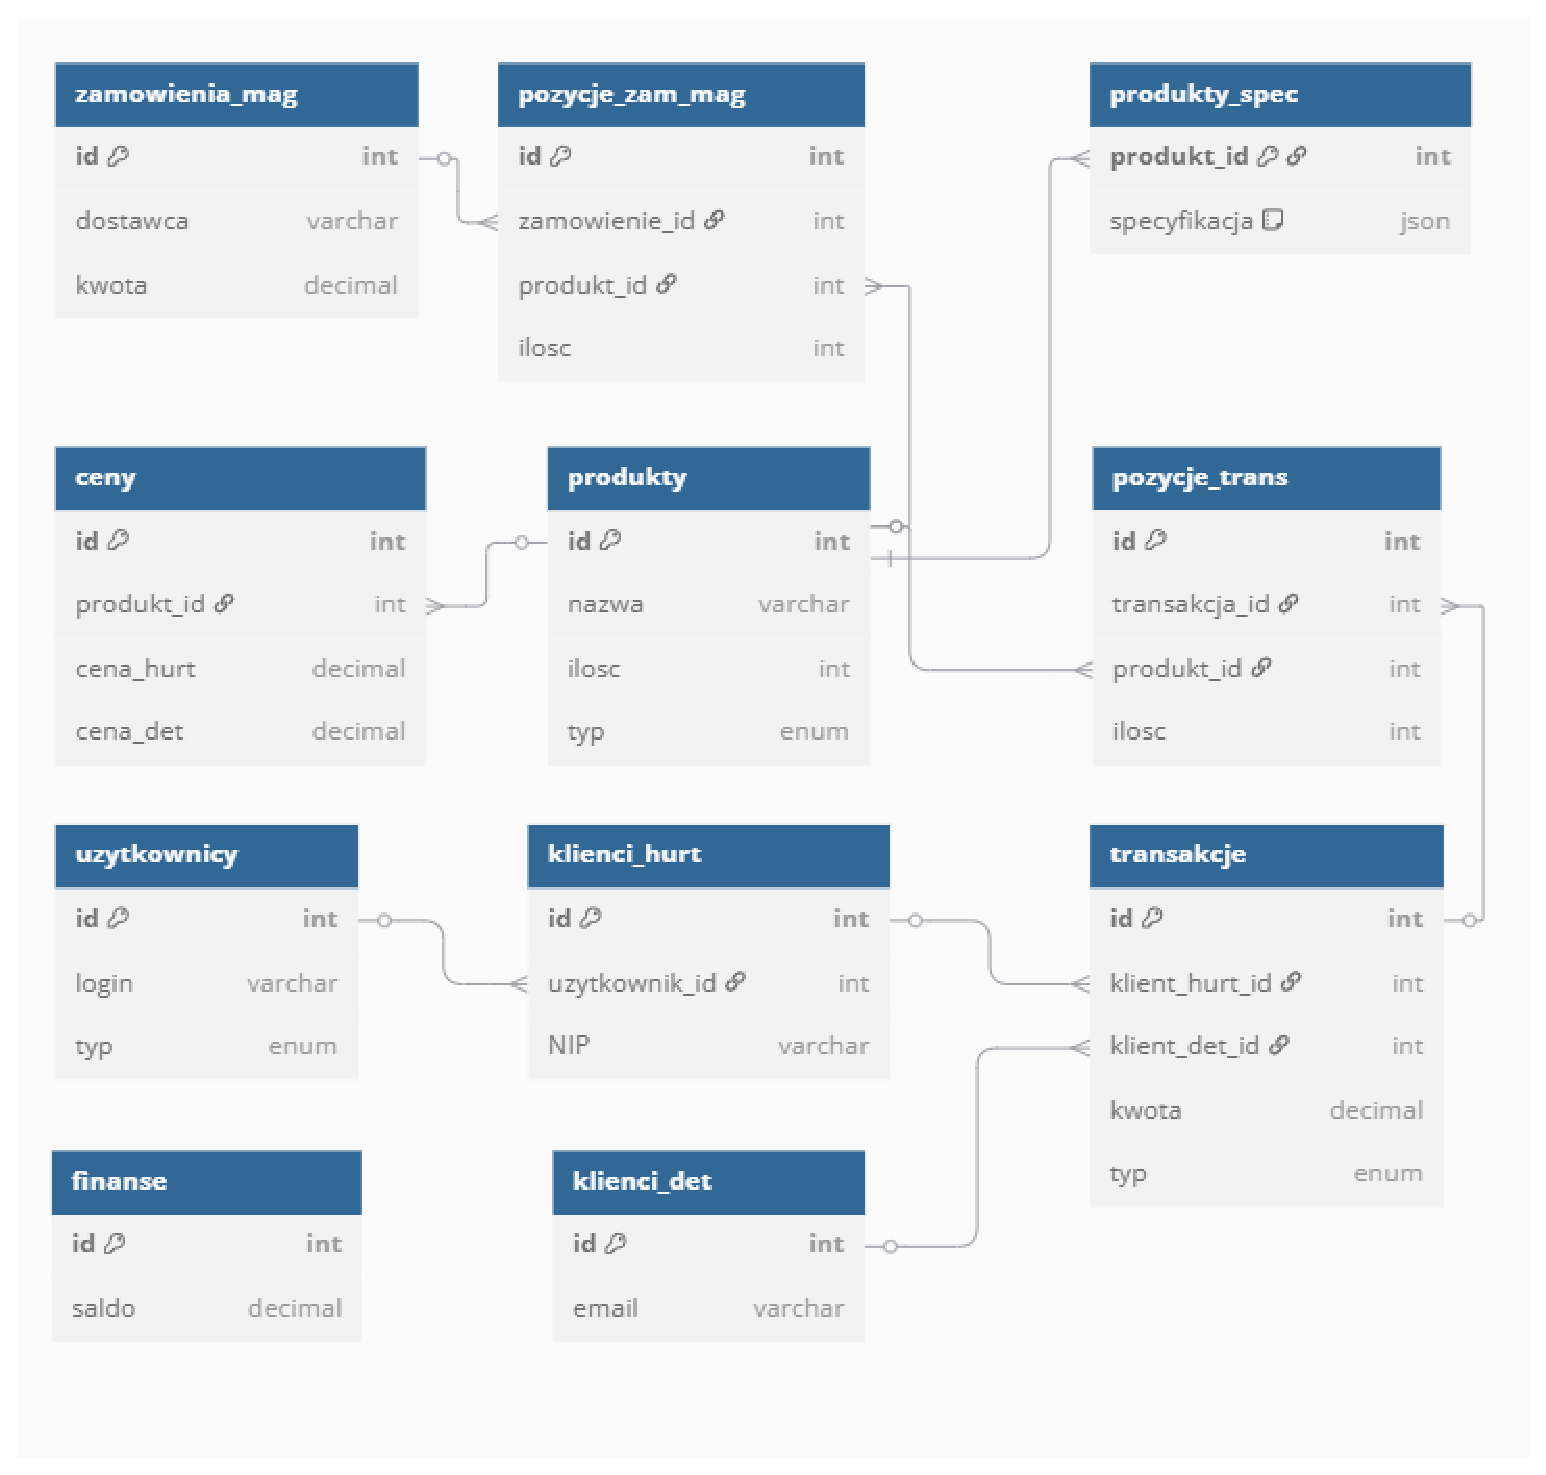
\includegraphics[width=\linewidth]{figures/fig_0001.eps}
    \caption{Schemat bazy danych (ERD) aplikacji sklepu.}
    \label{fig:erd_diagram}
    \small{Źródło: Wygenerowano za pomocą https://dbdiagram.io/}
\end{figure}
\clearpage

\section{Wymagania systemowe}
Uruchomienie projektu w środowisku deweloperskim wymaga zainstalowania i skonfigurowania dwóch głównych narzędzi. Do obsługi bazy danych niezbędny jest pakiet \textbf{XAMPP}, który dostarcza serwer Apache oraz MariaDB (kompatybilny z MySQL). Z kolei do kompilacji i uruchomienia kodu źródłowego aplikacji Java wymagane jest środowisko programistyczne \textbf{IntelliJ IDEA}. Aktualne wymagania systemowe dla obu programów dostępne są na ich oficjalnych stronach:
\begin{itemize}
    \item \textbf{XAMPP:} \url{https://www.apachefriends.org/download.html}
    \item \textbf{IntelliJ IDEA:} \url{https://www.jetbrains.com/help/idea/installation-guide.html#requirements}
\end{itemize}


\chapter{Harmonogram i Zarządzanie Projektem}
\label{chap:harmonogram}

\section{Harmonogram realizacji - Diagram Ganta}
\label{sec:gantt}

Proces tworzenia aplikacji został podzielony na kilka kluczowych etapów, których realizację w czasie ilustruje diagram Gantta (Rys. \ref{fig:gantt_chart}). Prace nad projektem rozłożono w sposób umożliwiający systematyczny postęp i iteracyjne dostarczanie funkcjonalności.

\begin{itemize}
    \item \textbf{Faza 1: Analiza i Projektowanie (ok. 15\% czasu pracy)}: Ten początkowy etap obejmował zdefiniowanie wymagań funkcjonalnych i niefunkcjonalnych , zaprojektowanie trójwarstwowej architektury systemu  oraz stworzenie schematu relacyjnej bazy danych w MySQL.
    
    \item \textbf{Faza 2: Implementacja Warstwy Danych i Logiki Biznesowej (ok. 30\% czasu pracy)}: Największą część tej fazy zajęło stworzenie warstwy dostępu do danych (DAO)  oraz klas modelu (np. \texttt{Product} , \texttt{Customer} ), które stanowią fundament komunikacji z bazą danych.
    
    \item \textbf{Faza 3: Implementacja Interfejsu Graficznego Użytkownika (ok. 40\% czasu pracy)}: Był to najbardziej czasochłonny etap, obejmujący budowę wszystkich okien i paneli aplikacji w technologii Java Swing (np. \texttt{AdminForm} , \texttt{ShopRetailForm} ) , implementację logiki obsługi zdarzeń (np. kliknięcia przycisków)  oraz stylizację komponentów w celu zapewnienia spójnego i intuicyjnego interfejsu.
    
    \item \textbf{Faza 4: Testowanie i Dokumentacja (ok. 15\% czasu pracy)}: Ostatni etap poświęcono na manualne testy kluczowych scenariuszy użytkowania, takich jak proces logowania , składanie zamówień  czy zarządzanie danymi przez administratora. Równolegle tworzono niniejszą dokumentację techniczną w systemie \LaTeX.
\end{itemize}

\begin{figure}[H]
    \centering
    \includegraphics[width=\linewidth]{figures/fig_0008.eps}
    \caption{Harmonogram realizacji projektu (Diagram Ganta).}
    \label{fig:gantt_chart}
    \small{Źródło: Opracowanie własne na podstawie szablonu Microsoft Gantt Chart Template.}
\end{figure}

\section{Napotkane wyzwania i rozwiązania}
W trakcie prac nad projektem nie obyło się bez pewnych trudności, które wymagały kreatywnego podejścia. Jednym z wyzwań była implementacja intuicyjnego mechanizmu wyboru daty w panelu administratora. Początkowe rozwiązanie, oparte na standardowych komponentach biblioteki Swing, takich jak \texttt{JComboBox} dla miesiąca i roku oraz \texttt{JButton} dla dni, okazało się nieestetyczne i mało wygodne dla użytkownika.

W poszukiwaniu lepszej alternatywy przeprowadzono research w internecie, w tym na platformie GitHub, w celu znalezienia gotowej biblioteki z komponentem kalendarza. Ostatecznie wybór padł na bibliotekę \texttt{LGoodDatePicker} \cite{LGoodDatePicker}. Jej integracja z projektem była strzałem w dziesiątkę. Biblioteka dostarczyła atrakcyjny wizualnie i prosty w obsłudze kalendarz, co znacząco poprawiło użyteczność aplikacji w miejscach wymagających operowania na datach, łącząc funkcjonalność z nowoczesnym wyglądem.

\section{System kontroli wersji i repozytorium}
Zarządzanie kodem źródłowym projektu opierało się na systemie kontroli wersji **Git**, który jest standardem w nowoczesnym wytwarzaniu oprogramowania. Wszystkie operacje, takie jak tworzenie commitów, zarządzanie gałęziami (branching) czy scalanie zmian (merging), były wykonywane przy użyciu zintegrowanego klienta Git w środowisku programistycznym **IntelliJ IDEA**.

Jako centralne, zdalne repozytorium kodu wykorzystano platformę **GitHub**. Cały projekt, wraz z historią zmian, jest publicznie dostępny pod adresem:
\begin{center}
    \url{https://github.com/Deskalisko/Projekt_JAVA}
\end{center}
Wykorzystanie systemu kontroli wersji pozwoliło na systematyczne śledzenie postępów, bezpieczne eksperymentowanie z nowymi funkcjonalnościami w osobnych gałęziach oraz zapewniło stałą kopię zapasową projektu.

\clearpage


\chapter{Prezentacja warstwy użytkowej projektu}
\label{chap:warstwa_uzytkowa}
W niniejszym rozdziale zaprezentowano warstwę użytkową projektu, czyli graficzny interfejs użytkownika (GUI), z którym wchodził w interakcję użytkownik końcowy. Opisano kluczowe widoki aplikacji, w tym ekran główny, panele zakupowe dla klientów detalicznych i hurtowych oraz moduły panelu administratora.

\section{Ekran Główny i Proces Logowania}
Punktem startowym aplikacji jest ekran główny (\texttt{MainForm.java}), przedstawiony na Rys. \ref{fig:main_form}, który pełni rolę centrum nawigacyjnego. Z jego poziomu użytkownik może przejść do przeglądania listy produktów, rozpocząć proces zakupowy lub zalogować się do systemu. Panel logowania jest kluczowym elementem, który na podstawie wprowadzonych danych uwierzytelnia użytkownika i kieruje go do odpowiedniego modułu aplikacji. Zaimplementowano również funkcjonalność resetowania hasła, która po weryfikacji tożsamości użytkownika pozwala na ustawienie nowego hasła.

\begin{figure}[H]
    \centering
    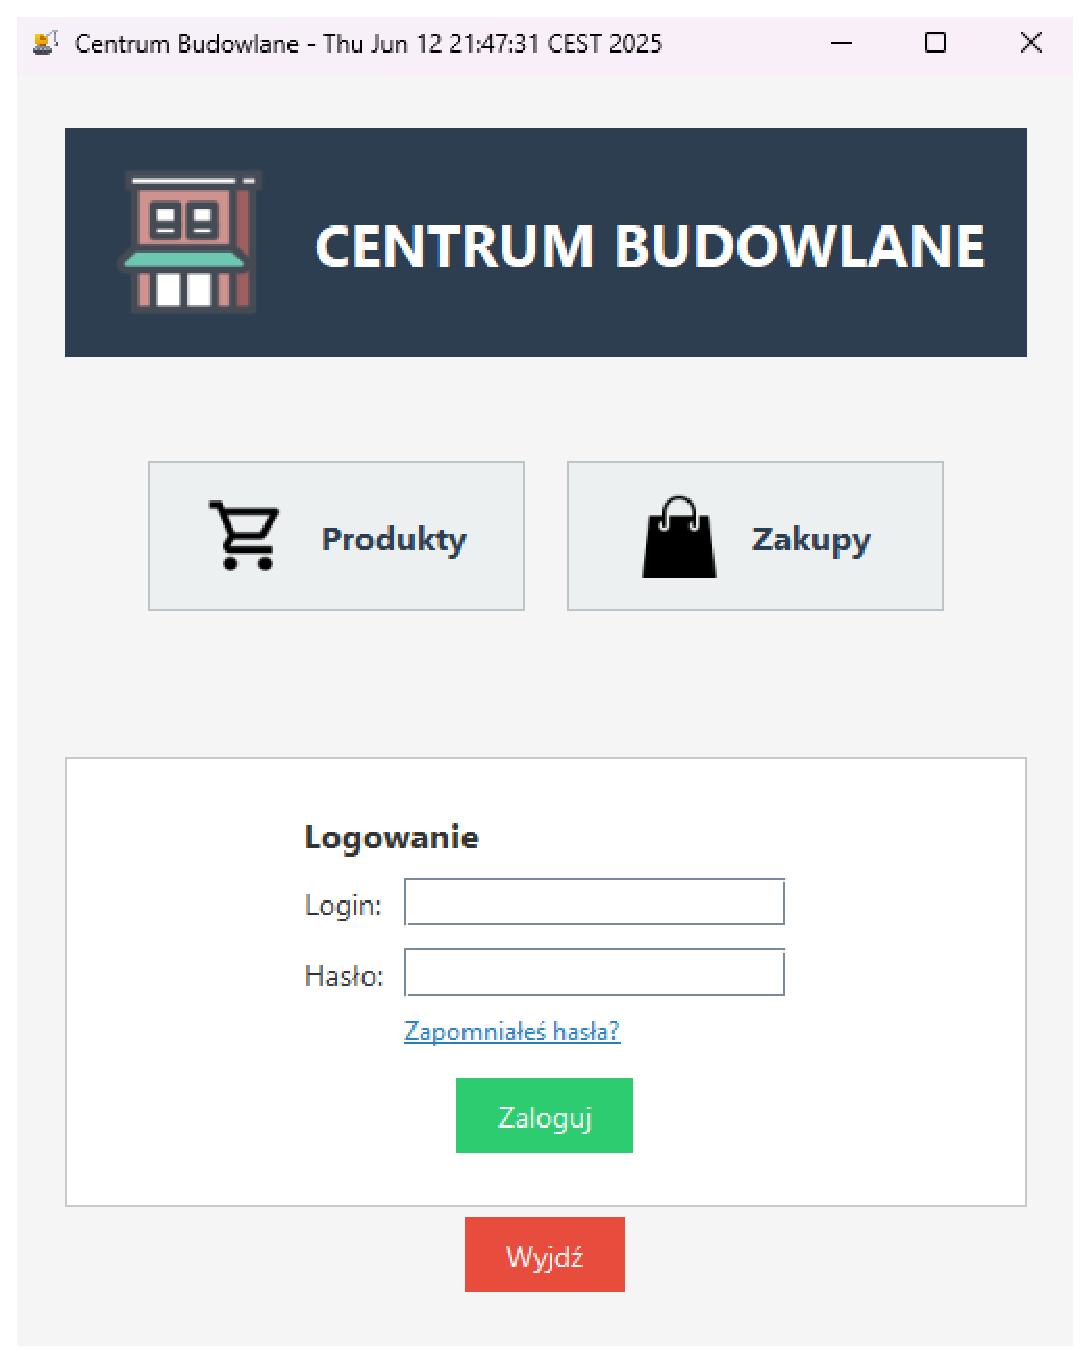
\includegraphics[width=0.6\linewidth]{figures/fig_0010.eps} 
    \caption{Główny ekran aplikacji z widocznym panelem logowania.}
    \label{fig:main_form}
    \small{Źródło: Opracowanie własne}
\end{figure}
\clearpage

\section{Interfejs Klienta}
Interfejs przeznaczony dla klienta został zaprojektowany z myślą o intuicyjności i wygodzie procesu zakupowego. Mimo że logika biznesowa i wygląd paneli dla klienta detalicznego (\texttt{ShopRetailForm.java}) i hurtowego (\texttt{ShopWholeSaleForm.java}) są do siebie bardzo zbliżone, istnieją między nimi kluczowe różnice.

\subsection{Panel Klienta Detalicznego}
Główny widok sklepu dla klienta detalicznego (Rys. \ref{fig:shop_retail}) składa się z trzech głównych sekcji: panelu danych klienta, listy dostępnych produktów oraz panelu koszyka. Klient może swobodnie przeglądać produkty, dodawać je do koszyka za pomocą przycisku i dedykowanego pola `JSpinner` do określania ilości , a następnie sfinalizować zamówienie. Kluczową cechą tego modułu jest to, że klient nie musi posiadać konta w systemie. Dane do wysyłki podawane są jednorazowo w oknie dialogowym `AddEditRetailCustomer`, które jest wywoływane przed złożeniem zamówienia.

\begin{figure}[H]
    \centering
    \includegraphics[width=0.85\linewidth]{figures/fig_0002.eps}
    \caption{Widok panelu zakupowego dla klienta detalicznego.}
    \label{fig:shop_retail}
    \small{Źródło: Opracowanie własne}
\end{figure}

\clearpage

\subsection{Panel Klienta Hurtowego}
Panel klienta hurtowego (\texttt{ShopWholeSaleForm.java}) jest wizualnie niemal identyczny z panelem detalicznym, jednak dostosowany do specyfiki klienta biznesowego. Główne różnice to:
\begin{itemize}
    \item \textbf{Ceny hurtowe:} Tabela produktów automatycznie ładuje niższe ceny hurtowe pobierane z bazy danych.
    \item \textbf{Stałe dane klienta:} Dane klienta, takie jak nazwa firmy czy NIP, są ładowane automatycznie po zalogowaniu i wyświetlane w górnej części panelu, co eliminuje potrzebę ich każdorazowego wprowadzania. Klient ma możliwość edycji swoich danych oraz zmiany hasła.
    \item \textbf{Warunki zamówienia:} System waliduje, czy zamówienie hurtowe spełnia minimalne progi, takie jak łączna liczba produktów w koszyku (minimum 3) oraz minimalna wartość zamówienia (50 zł).
\end{itemize}

\section{Panel Administratora}
Panel administratora (\texttt{AdminForm.java}) stanowi centrum dowodzenia aplikacją. Jest to główny pulpit, z którego administrator ma bezpośredni dostęp do wszystkich kluczowych modułów zarządczych. Został zaprojektowany w sposób modułowy, aby zapewnić szybki i intuicyjny dostęp do poszczególnych funkcjonalności. W centralnej części panelu wyświetlana jest tabela z listą ostatnich transakcji, co pozwala na bieżące monitorowanie aktywności w sklepie.

\begin{figure}[H]
    \centering
    \includegraphics[width=0.85\linewidth]{figures/fig_0011.eps}
    \caption{Główny widok panelu administratora.}
    \label{fig:admin_form}
    \small{Źródło: Opracowanie własne}
\end{figure}

Główne moduły, dostępne za pomocą dedykowanych przycisków, to:
\begin{itemize}
    \item \textbf{Zarządzanie Klientami} (\texttt{CustomerList.java})
    \item \textbf{Zarządzanie Magazynem} (\texttt{WarehouseForm.java})
    \item \textbf{Zarządzanie Transakcjami} (\texttt{ManagementTransactionForm.java})
\end{itemize}
Poniżej opisano szczegółowo działanie każdego z tych modułów.

\subsection{Zarządzanie Klientami i ich szczegóły}
Moduł \texttt{CustomerList.java} pozwala na przeglądanie, dodawanie (tylko hurtowych), edytowanie oraz usuwanie klientów. Za pomocą przełączników `JRadioButton` administrator może płynnie przełączać się między listą klientów detalicznych a hurtowych, a dane w tabeli są dynamicznie odświeżane.

Kluczową funkcjonalnością tego panelu jest możliwość wglądu w szczegółowe dane klienta po naciśnięciu przycisku "Szczegóły". Otwiera to nowe okno (\texttt{CustomerDetails.java}), które prezentuje kompleksowe informacje na temat wybranego klienta w trzech osobnych zakładkach:
\begin{itemize}
    \item \textbf{Informacje ogólne:} Wyświetlane są tu podstawowe dane, takie jak imię i nazwisko, typ klienta (detaliczny/hurtowy), łączna suma zakupów, adres oraz dane kontaktowe (telefon, e-mail, a w przypadku klienta hurtowego również NIP i nazwa firmy).
    \item \textbf{Historia transakcji:} Tabela zawierająca listę wszystkich transakcji dokonanych przez danego klienta, wraz z datą, kwotą, typem i listą zakupionych produktów.
    \item \textbf{Statystyki produktów:} Tabela grupująca wszystkie produkty zakupione przez klienta, przedstawiająca sumaryczną ilość oraz łączną wartość dla każdego z nich.
\end{itemize}

\begin{figure}[H]
    \centering
    \includegraphics[width=0.8\linewidth]{figures/fig_0012.eps}
    \caption{Panel szczegółowych informacji o kliencie.}
    \label{fig:customer_details}
    \small{Źródło: Opracowanie własne}
\end{figure}
\clearpage

\subsection{Zarządzanie Magazynem}
Widok magazynu (\texttt{WarehouseForm.java}) jest interfejsem bardzo zbliżonym wizualnie do panelu zarządzania klientami, jednak w pełni dostosowanym do operacji na produktach. Udostępnia narzędzia do pełnej kontroli nad asortymentem, pozwalając administratorowi na przeglądanie stanów magazynowych, sortowanie i filtrowanie danych (np. wyświetlając tylko produkty, których ilość jest niska), a także edytowanie ilości sztuk danego produktu. Zaimplementowano tu również funkcję składania zamówień do dostawców (\texttt{createWarehouseOrder}) oraz generowania raportów o niskich stanach magazynowych w formacie CSV. W panelu wyświetlane jest także aktualne saldo finansowe sklepu, które jest modyfikowane przy każdym zamówieniu magazynowym.

\subsection{Zarządzanie Transakcjami}
Ostatni moduł, \texttt{ManagementTransactionForm.java}, służy do przeglądania i analizy wszystkich transakcji w systemie. Administrator może filtrować transakcje według typu (detaliczne, hurtowe) oraz zakresu dat, korzystając z zintegrowanego komponentu kalendarza \texttt{LGoodDatePicker} \cite{LGoodDatePicker}. Po wybraniu transakcji z tabeli, w dedykowanym panelu wyświetlane są jej szczegółowe dane, w tym lista zakupionych produktów. Panel ten umożliwia również generowanie raportów CSV z przefiltrowanych danych.

\begin{figure}[H]
    \centering
    \includegraphics[width=0.85\linewidth]{figures/fig_0007.eps}
    \caption{Widok panelu zarządzania transakcjami z zintegrowanym kalendarzem.}
    \label{fig:management_transaction}
    \small{Źródło: Opracowanie własne}
\end{figure}
\clearpage


\chapter{Testowanie aplikacji}

W niniejszym rozdziale przedstawiono proces testowania aplikacji, zarówno w aspekcie manualnym. Testowanie ma na celu weryfikację poprawności działania wszystkich funkcjonalności systemu, sprawdzenie jego stabilności oraz zapewnienie pozytywnych doświadczeń użytkownika.

\section{Testowanie manualne}
Testowanie manualne stanowi kluczowy etap w zapewnieniu jakości aplikacji, zwłaszcza w przypadku interfejsów graficznych (GUI). Polega ono na interakcji z programem z perspektywy końcowego użytkownika, pozwalając na wykrycie problemów z użytecznością, wizualną spójnością oraz błędów, które mogą być trudne do zidentyfikowania za pomocą testów automatycznych. Poniżej przedstawiono wybrane scenariusze testowe, które zostały przeprowadzone manualnie.
\clearpage

\begin{minipage}{\linewidth}
\subsection{Testy scenariuszy logowania i rejestracji}
Kluczowym elementem każdego systemu jest bezpieczne i poprawne zarządzanie kontami użytkowników. Manualne testy tej sekcji obejmowały:
\begin{itemize}
    \item Pomyślne logowanie dla istniejącego użytkownika (klienta detalicznego i administratora).
    \item Logowanie z błędnymi danymi (niepoprawna nazwa użytkownika, niepoprawne hasło).
    \item Testowanie walidacji pól formularza logowania (np. puste pola).
    \item Próba rejestracji użytkownika z istniejącą nazwą użytkownika lub adresem e-mail.
    \item Weryfikacja wyświetlanych komunikatów o błędach. Przykład takiego komunikatu, który informuje o błędnie wprowadzonych danych logowania, widoczny jest na Rysunku \ref{fig:bledne_logowanie}.
\end{itemize}

\begin{figure}[H]
    \centering
    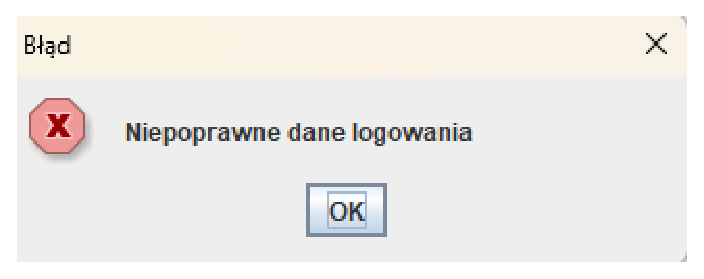
\includegraphics[width=0.5\linewidth]{figures/fig_0004.eps}
    \caption{Komunikat o błędnym wprowadzeniu danych logowania. }
    \label{fig:bledne_logowanie}
    \small{Źródło: Opracowanie własne}
\end{figure}
\end{minipage}

\vspace{1cm}

% --- Blok 2: Opis + Rysunek 4.2 ---
\begin{minipage}{\linewidth}
\subsection{Testy procesu zamawiania dla klienta detalicznego}
Szczególną uwagę zwrócono na poprawność procesu składania zamówienia przez klienta detalicznego. Obejmowało to:
\begin{itemize}
    \item Dodawanie różnych produktów do koszyka i weryfikacja poprawności sumy.
    \item Usuwanie produktów z koszyka i zmiana ich ilości.
    \item Finalizacja zamówienia z poprawnymi danymi klienta (imię, nazwisko, adres, telefon, e-mail).
    \item Testowanie walidacji pól formularza zamówienia (np. puste pola, niepoprawny format e-maila/telefonu). Na Rysunku \ref{fig:bledne_dane_zamowienia} przedstawiono przykład sytuacji, w której dane są niekompletne lub zawierają nieprawidłowe dane, co skutkuje wyświetleniem błędu.
\end{itemize}

\begin{figure}[H]
    \centering
    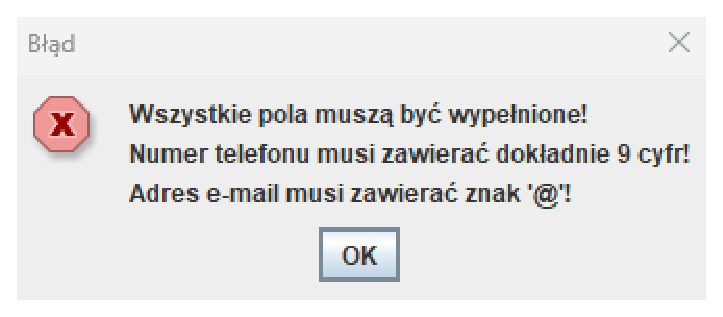
\includegraphics[width=0.5\linewidth]{figures/fig_0005.eps}
    \caption{Przykład błędnego wprowadzenia danych przez klienta detalicznego.}
    \label{fig:bledne_dane_zamowienia}
    \small{Źródło: Opracowanie własne}
\end{figure}
\end{minipage}

\vspace{1cm}


\begin{minipage}{\linewidth}
\subsection{Testy specyficznych scenariuszy klienta hurtowego}
Dla klienta hurtowego przeprowadzono dodatkowe testy, uwzględniające specyfikę jego uprawnień:
\begin{itemize}
    \item Sprawdzenie, czy ceny produktów są wyświetlane jako ceny hurtowe.
    \item Próba złożenia zamówienia z pustym koszykiem. Komunikat informujący o tej sytuacji jest widoczny na Rysunku \ref{fig:pusty_koszyk}.
    \item Testowanie złożenia zamówienia, które nie spełnia minimalnego wymogu dla zamówień hurtowych (jeśli taki istnieje w aplikacji).
    \item Walidacja, czy system odpowiednio reaguje na próby zamówienia zbyt małej ilości produktów.
\end{itemize}

\begin{figure}[H]
    \centering
    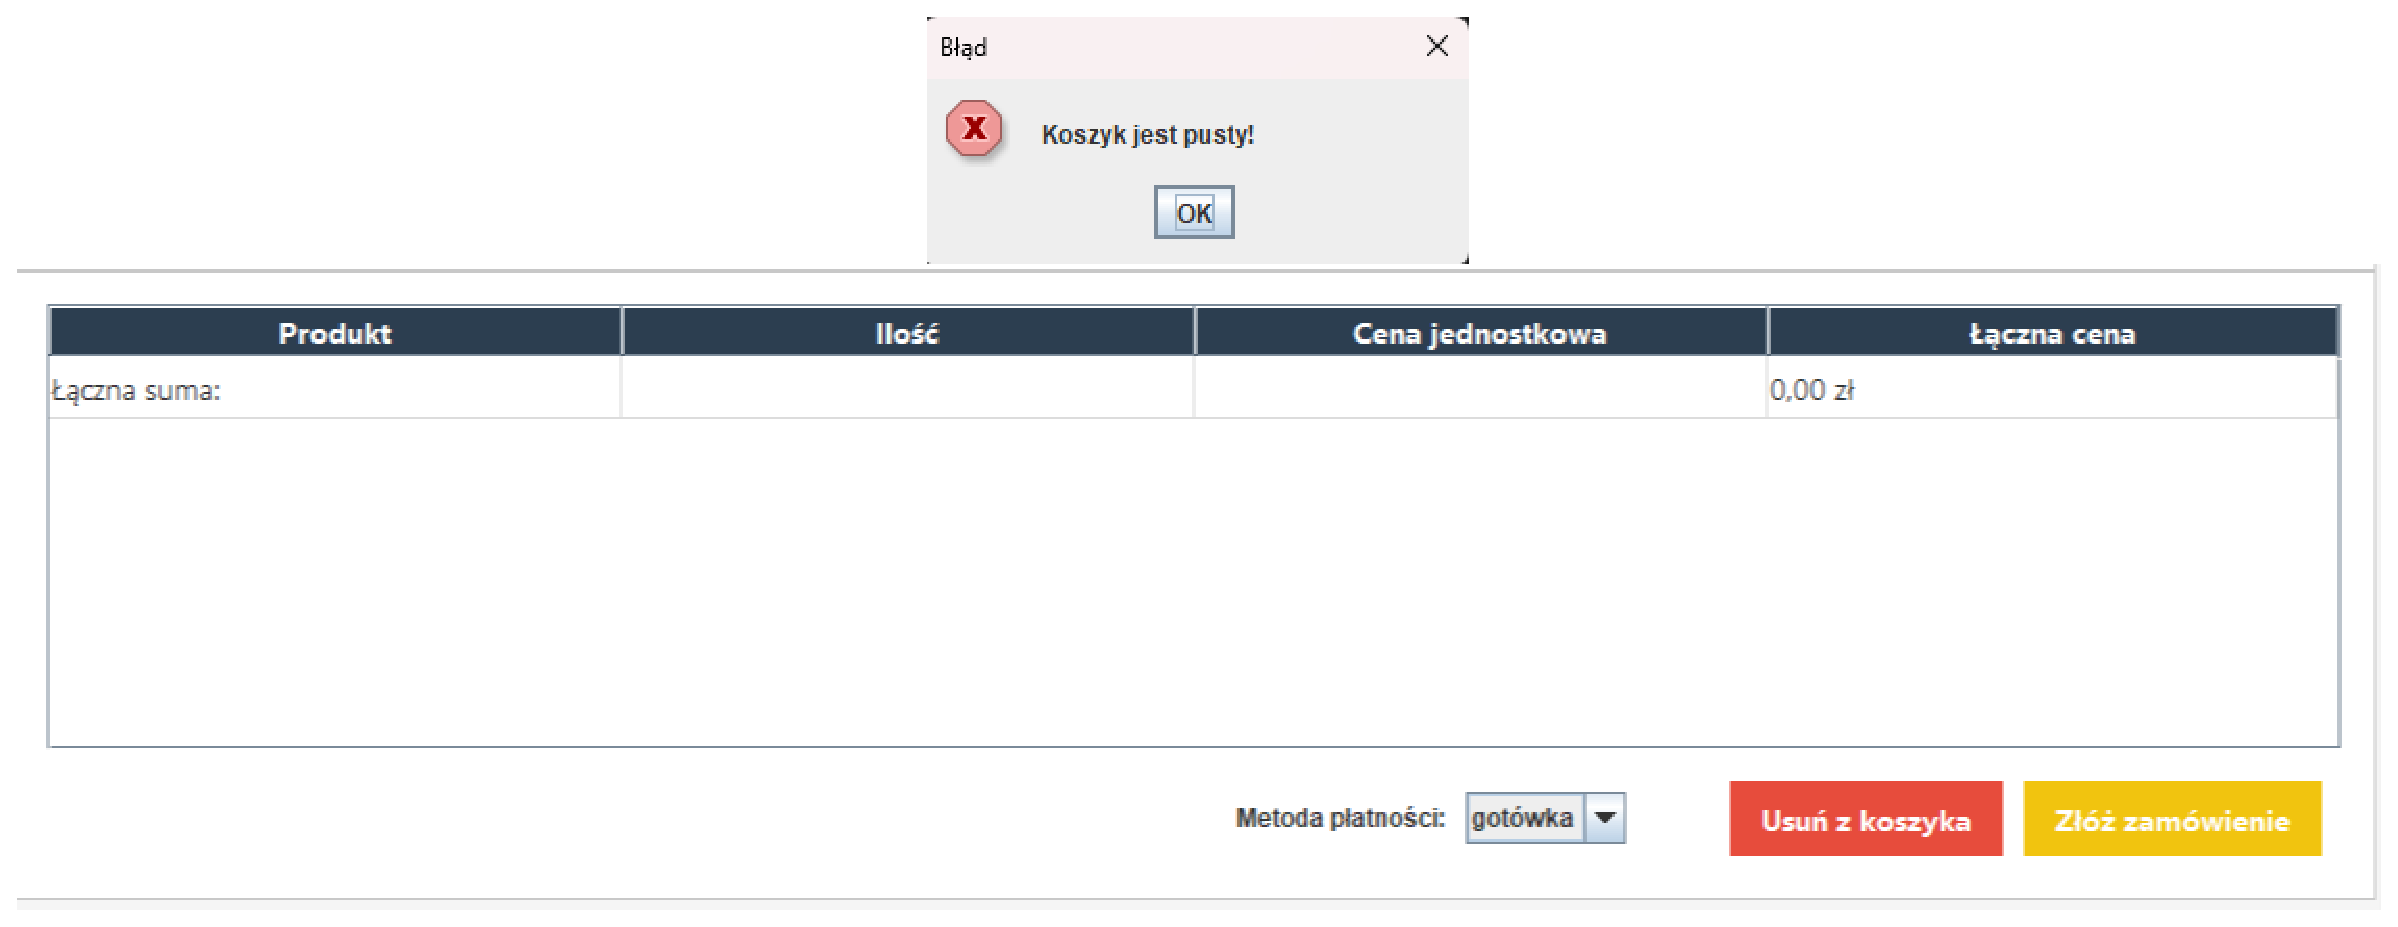
\includegraphics[width=\linewidth]{figures/fig_0006.eps}
    \caption{Komunikat informujący o próbie złożenia zamówienia z pustym koszykiem. }
    \label{fig:pusty_koszyk}
    \small{Źródło: Opracowanie własne}
\end{figure}
\end{minipage}

\subsection{Testy walidacji pól i zabezpieczeń}
W aplikacji zaimplementowano szereg zabezpieczeń i walidacji, które zostały dokładnie przetestowane manualnie. Szczególną uwagę zwrócono na:

\begin{itemize}
    \item Sprawdzenie, czy pola przeznaczone na wartości liczbowe (np. ilość produktów, cena) prawidłowo odrzucają próby wprowadzenia tekstu i akceptują tylko cyfry.
    \item Weryfikację formatu wprowadzanych danych, takich jak adresy e-mail (muszą zawierać znak ‘@’) oraz numery telefonów (muszą składać się z 9 cyfr).
    \item Przetestowanie mechanizmu zmiany hasła, w którym sprawdzono, czy system wymusza identyczność haseł w polach ``nowe hasło'' i ``powtórz nowe hasło''. W przypadku niezgodności, aplikacja wyświetlała odpowiedni komunikat o błędzie.
    \item Dokładne przetestowanie komponentu wyboru daty, LGoodDatePicker \cite{LGoodDatePicker}. Weryfikacja objęła otwieranie i zamykanie kalendarza, wybór daty, ręczne wprowadzanie oraz obsługę błędnych formatów.
    \item Symulację utraty połączenia z bazą danych, aby sprawdzić, czy aplikacja w takiej sytuacji nie ulega awarii, lecz wyświetla użytkownikowi zrozumiały komunikat o problemie.
\end{itemize}
\chapter{Implementacja i Kluczowe Fragmenty Kodu}
\section{Wybrane Metody Usprawniające Pracę}

\begin{minipage}{\linewidth}
\subsection{Metoda `createStyledButton` - Ujednolicenie Wyglądu Przycisków}
Metoda `createStyledButton` jest przykładem dobrej praktyki programistycznej, pozwalającej na tworzenie spójnych stylistycznie przycisków w interfejsie użytkownika. Dzięki niej unika się powielania kodu odpowiedzialnego za ustawianie czcionki, kolorów, ramek i innych właściwości wizualnych dla każdego przycisku z osobna. Znacząco przyspieszyło to budowanie interfejsu graficznego. 

\lstinputlisting[style=javaStyle, language=Java, caption=Metoda createStyledButton, label=lst:createStyledButton]{src/CreateStyledButton.java}
\end{minipage}

\vspace{1cm}

\begin{minipage}{\linewidth}
\subsection{Metoda `getConnection` - Efektywne Zarządzanie Połączeniami z Bazą Danych}
Zarządzanie połączeniami z bazą danych jest kluczowe dla wydajności i niezawodności aplikacji.  Metoda `getConnection` z klasy `DatabaseConnection` zapewnia scentralizowany i prosty sposób na uzyskanie aktywnego połączenia z bazą danych MySQL.  Jej wykorzystanie znacznie uprościło operacje na danych, minimalizując ryzyko błędów związanych z otwieraniem i zamykaniem połączeń. 

\lstinputlisting[style=javaStyle, language=Java, caption=Metoda getConnection, label=lst:getConnection]{src/DatabaseConnection.java}
\end{minipage}

\section{Inne Istotne Fragmenty Kodu}

\begin{minipage}{\linewidth}
\subsection{Integracja i Użycie Kalendarza \texttt{JDateChooser}}
W celu ułatwienia wyboru daty, komponent \texttt{JDateChooser} został zintegrowany z interfejsem użytkownika. Jest to szczególnie przydatne **w panelu zarządzania transakcjami administratora, gdzie umożliwia precyzyjne filtrowanie i wyszukiwanie transakcji według daty**. Komponent ten eliminuje konieczność ręcznego wprowadzania daty i ryzyko błędów formatowania, zapewniając jednocześnie spójny wygląd i format daty w całej aplikacji, a także w innych miejscach, gdzie wybór daty jest istotny. 
Finalny wygląd panelu z zaimplementowanym komponentem kalendarza przedstawiono na \figurename~\ref{fig:management_transaction}.

\lstinputlisting[style=javaStyle, language=Java, caption=Metoda createDateChooser, label=lst:createDateChooser]{src/CreateDateChooser.java}

\end{minipage}

\chapter{Podsumowanie}
\label{chap:podsumowanie}

\section{Wnioski}
Zrealizowany projekt zakończył się sukcesem, osiągając główny cel, którym było stworzenie w pełni funkcjonalnej, dwumodułowej aplikacji desktopowej do zarządzania sklepem. System, oparty o technologie Java, Swing oraz bazę danych MySQL, poprawnie realizuje wszystkie kluczowe założenia, oferując zarówno panel przeznaczony dla klienta, jak i rozbudowane centrum zarządcze dla administratora.

Zastosowanie trójwarstwowej architektury z wzorcem projektowym DAO (Data Access Object) okazało się kluczowe dla zapewnienia czystości i skalowalności kodu. Udało się skutecznie oddzielić warstwę prezentacji od logiki biznesowej i dostępu do danych, co ułatwiło implementację, testowanie oraz potencjalny dalszy rozwój poszczególnych komponentów systemu.

Wszystkie zdefiniowane wymagania funkcjonalne, takie jak proces logowania, zarządzanie asortymentem i stanami magazynowymi, obsługa koszyka zakupowego oraz finalizacja transakcji, zostały pomyślnie zaimplementowane i zweryfikowane w testach manualnych. Aplikacja stanowi solidną i kompletną podstawę, która może być w przyszłości rozwijana o nowe, zaawansowane funkcjonalności.

\section{Propozycje dalszego rozwoju}
Mimo że obecna wersja aplikacji jest w pełni funkcjonalna, istnieje znaczny potencjał do jej dalszej rozbudowy. Poniżej przedstawiono trzy kluczowe kierunki możliwego rozwoju:

\begin{enumerate}
    \item \textbf{Wdrożenie testów automatycznych:} W celu podniesienia niezawodności i ułatwienia przyszłego utrzymania kodu, kluczowym krokiem byłoby wprowadzenie testów automatycznych. Przy użyciu frameworka \textbf{JUnit} oraz bibliotek takich jak \textbf{Mockito}, można by stworzyć testy jednostkowe dla klas w warstwie DAO, weryfikując poprawność operacji bazodanowych w izolacji. Umożliwiłoby to szybkie wykrywanie regresji po wprowadzeniu nowych zmian.

    \item \textbf{Rozbudowa modułu raportowania i analiz:} Obecny system generuje podstawowe raporty w formacie CSV. Znacznym usprawnieniem byłoby stworzenie zaawansowanego modułu analitycznego, który wizualizowałby dane za pomocą wykresów (np. z wykorzystaniem biblioteki \textbf{JFreeChart}). Moduł ten mógłby generować raporty sprzedaży w ujęciu czasowym, analizować najpopularniejsze produkty czy przedstawiać statystyki dotyczące aktywności poszczególnych klientów.

    \item \textbf{Funkcjonalność resetowania hasła dla użytkowników:} Wdrożenie bezpiecznego mechanizmu resetowania hasła, co zwiększyłoby użyteczność i bezpieczeństwo aplikacji dla użytkowników końcowych. Wymagałoby to m.in. implementacji wysyłki wiadomości e-mail z linkiem do resetowania oraz odpowiedniej obsługi po stronie serwera.
\end{enumerate}


% ********** Koniec **********


% Wyłączenie działania `ulem` na czas bibliografii
\renewcommand{\emph}[1]{\textit{#1}}
% Bibliografia
% Dodanie bibliografi do spisu treści
\phantomsection % <-- DODANE: Tworzy kotwicę dla linku
\addcontentsline{toc}{section}{\textbf{Bibliografia}}
\bibliographystyle{plain}
\bibliography{bibliografia}

% Przywrócenie działania `ulem`
\renewcommand{\emph}[1]{\uline{#1}}



\clearpage
% Dodanie spisu rysunków do spisu treści
\phantomsection % <-- DODANE: Tworzy nową, poprawną kotwicę
\addcontentsline{toc}{section}{\textbf{Spis rysunków}}
\listoffigures
\clearpage

\clearpage

% Dodanie spisu listingow do spisu treści
\phantomsection % <-- DODANE: Tworzy nową, poprawną kotwicę
\addcontentsline{toc}{section}{\textbf{Spis listingów}}
\lstlistoflistings
\clearpage

% \appendix
\chapter*{}
\label{cha:statement-A}
\makeatletter
\addcontentsline{toc}{section}{\textbf{Oświadczenie studenta o samodzielności pracy}}

\noindent
\begin{flushright}
    \begin{minipage}[!h]{10cm}
        Załącznik nr 2 do Zarządzenia nr 228/2021 Rektora Uniwersytetu Rzeszowskiego z dnia 1 grudnia 2021 roku w sprawie ustalenia procedury antyplagiatowej w Uniwersytecie Rzeszowskim
    \end{minipage}
\end{flushright}

\begin{center}
    \vspace*{10mm}
    \noindent  {\textbf{OŚWIADCZENIE STUDENTA O SAMODZIELNOŚCI PRACY} }
    \vspace*{10mm}
\end{center}

\noindent
\dotuline{\hspace{1.3cm}\@author\hspace{1.3cm}}\\
{\small Imię (imiona) i nazwisko studenta }\\

\noindent \@faculty\\

\noindent \dotuline{\hspace{1.4cm}\@degreeprogramme \hspace{1.4cm}}\\
{\small Nazwa kierunku} \\

\noindent \dotuline{\hspace{1.8cm}\@noAlbum\hspace{1.9cm}}\\
{\small Numer albumu}

\begin{enumerate}
    \item Oświadczam, że moja praca projektowa pt.: \@titlePL
          \begin{enumerate}[label=\arabic*)]
              \item została przygotowana przeze mnie samodzielnie*,
              \item nie narusza praw autorskich w rozumieniu ustawy z dnia 4 lutego 1994 roku o prawie autorskim i prawach pokrewnych (t.j. Dz.U. z 2021 r., poz. 1062) oraz dóbr osobistych chronionych prawem cywilnym,
              \item nie zawiera danych i informacji, które uzyskałem/am w sposób niedozwolony,
              \item nie była podstawą otrzymania oceny z innego przedmiotu na uczelni wyższej ani mnie, ani innej osobie.
          \end{enumerate}
    \item Jednocześnie wyrażam zgodę/nie wyrażam zgody** na udostępnienie mojej pracy projektowej do celów naukowo--badawczych z poszanowaniem przepisów ustawy o prawie autorskim i prawach pokrewnych.
\end{enumerate}


\vspace*{10mm}

\noindent
\underline{\hspace{6cm}} \hfill \underline{\hspace{6cm}} \\ 
\hspace*{13mm}(miejscowość, data)  \hspace*{63mm}(czytelny podpis studenta)
\vspace*{10mm}

\vfill
\noindent
* Uwzględniając merytoryczny wkład prowadzącego przedmiot \\
** -- niepotrzebne skreślić


\end{document}